\documentclass{article}

% Packages
\usepackage[margin=0.8in]{geometry}
\usepackage[utf8]{inputenc}
\usepackage{dsfont}
\usepackage{pgfplots}
\usepackage{algorithm}
\usepackage{algorithmic}
\usepackage{amsmath}
\usepackage{amsfonts}\usepackage{titling}
\renewcommand\maketitlehooka{\null\mbox{}\vfill}
\renewcommand\maketitlehookd{\vfill\null}

% Custom paragraph spacing
\setlength{\parskip}{0.75em}
\setcounter{section}{-1}

\title{Machine Learning -  Andrew Ng}
\author{Matteo Esposito}

% For page counter to start on p.2
\pagenumbering{gobble}

% Plot package backwards compatibility
\pgfplotsset{compat=1.14}

\begin{document}

    \begin{titlingpage}
        \maketitle
    \end{titlingpage}
    \newpage

    \section{Introduction}

        \textit{This document is a compilation of notes from the machine learning coursera MOOC taught by Prof. Andrew Ng of Stanford University
        offered by Coursera.}
        \par
        % Intro notes
        \textbf{Supervised learning} problems are categorized into "regression" and "classification" problems. In a regression problem, 
        we are trying to predict results within a continuous output, meaning that we are trying to map input variables to some 
        continuous function. In a classification problem, we are instead trying to predict results in a discrete output. In other words, 
        we are trying to map input variables into discrete categories.
        \par
        \textbf{Unsupervised learning} allows us to approach problems with little or no idea what our results should look like. 
        We can derive structure from data where we don't necessarily know the effect of the variables.
        We can derive this structure by clustering the data based on relationships among the variables in the data.
        With unsupervised learning there is no feedback based on the prediction results.
        \par
        From this point, we will use $X$ to denote the space of input values, and $Y$ to denote the space of output values. In this example, $X = Y = \mathbb{R}$.
        \par
        To describe the supervised learning problem slightly more formally, our goal is, given a training set, 
        to learn a function $h : X \longrightarrow Y$ so that $h(x)$ is a “good” predictor for the corresponding value of y. For historical reasons, this 
        function $h$ is called a hypothesis. 
        
        \subsection{Cost Function}
            
            We can measure the accuracy of our hypothesis function by using a \textbf{cost function}. This takes an average difference (actually a fancier version of an average)
            of all the results of the hypothesis with inputs from x's and the actual output y's.
            % Cost function
            \begin{align*}
               J(\theta_{0},\theta_{1}) = \frac{1}{2m}\sum_{i=1}^{m}(\hat{y_i} - y_i)^2 = \frac{1}{2m}\sum_{i=1}^{m}(h_{\theta}(x_i)- y_i)^2
            \end{align*}
            This function is otherwise called the "Squared error function", or "Mean squared error". The mean is halved $\left(\frac{1}{2}\right)$
            as a convenience for the computation of the gradient descent, as the derivative term of the square function will cancel out the $\left(\frac{1}{2}\right)$ 
            term. $J$ will be 0 if we can achieve a perfect fit (not always possible, and when possible, will probably mean overfitting). We can use a contour plot to visualize the minimizing of the cost function.
            % Contour plot
            \vspace{12pt}
            \begin{center}
                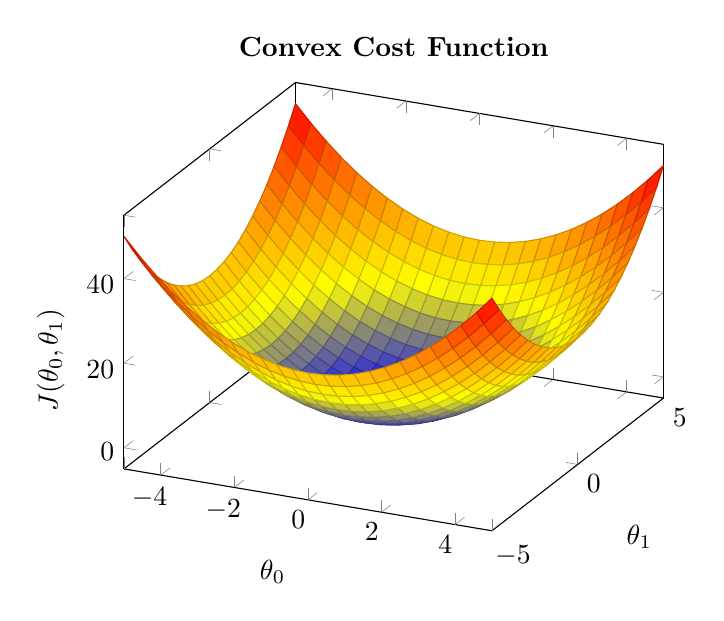
\begin{tikzpicture}
                    \begin{axis}[
                        title={\textbf{Convex Cost Function}},
                        xlabel = {$\theta_{0}$},
                        ylabel = {$\theta_{1}$},
                        zlabel = {$J(\theta_{0},\theta_{1})$}]
                        \addplot3[surf,] {x^2 + y^2};
                    \end{axis}
                \end{tikzpicture}
            \end{center}
            
        \subsection{Gradient Descent}

            \begin{algorithm}
                \caption{General Gradient Descent}
                \begin{algorithmic}
                    \FOR{$n >= 1$}
                        \STATE $n = $number of features, $m = $number of samples
                        \STATE \emph{repeat until convergence}:
                        \STATE \hspace{12pt}$\theta_j \gets \theta_j - \alpha\frac{\partial}{\partial\theta_j}J(\theta_{0},\theta_{1}) = \theta_j - \alpha\frac{1}{m}\sum_{i=1}^{m}(h_{\theta}(x^{(i)})-y^{(i)})x_{j}^{(i)}$
                    \ENDFOR
                \end{algorithmic}
            \end{algorithm}
            
            We will know that we have succeeded when our cost function is at the very bottom of the pits in our graph, i.e. when its value is the minimum. 
            
            The way we do this is by taking the derivative (the tangential line to a function) of our cost function. 
            The slope of the tangent is the derivative at that point and it will give us a direction to move towards.
            We make steps down the cost function in the direction with the steepest descent. 
            The size of each step is determined by the parameter $\alpha$, which is called the learning rate.

    \section{Linear Regression}

        \begin{algorithm}
            \caption{Gradient Descent for Linear Regression}
            \begin{algorithmic}
                \STATE $n = $number of features, $m = $number of samples
                \STATE \emph{repeat until convergence}:
                \STATE \hspace{12pt}$\theta_0 \gets \theta_0 - \alpha\frac{1}{m}\sum_{i=1}^{m}(h_{\theta}(x^{(i)})-y_i)$
                \STATE \hspace{12pt}$\theta_1 \gets \theta_1 - \alpha\frac{1}{m}\sum_{i=1}^{m}((h_{\theta}(x^{(i)})-y_i)x_{i})$
            \end{algorithmic}
        \end{algorithm}





    \section{Logistic Regression}



    \section{Neural Networks}


    \section{Neural Networks/Backpropagation}

\end{document}
